
%%%%%%%%%%%%%%%%%%%%%%%%%%%%%%%
%% Définition des commandes  %%
%%%%%%%%%%%%%%%%%%%%%%%%%%%%%%%%%%%%%%%%%%%%%%%%%%%%%%%%%%%%%%%%%%%%%%%%%%%%%
%% Toutes les commandes sont obligatoirement sous la forme \rsQuelqueChose %%
%%%%%%%%%%%%%%%%%%%%%%%%%%%%%%%%%%%%%%%%%%%%%%%%%%%%%%%%%%%%%%%%%%%%%%%%%%%%%

%%%%%%%%%%%%%%%%%%%%%%%%%%%%%
%% Note de frais seulement %%
%%%%%%%%%%%%%%%%%%%%%%%%%%%%%%%%%%%%%%%%%%%%%%%%%%%%%%%%%%%%%%%%%%%%%%%%%%%%%%%%%%%%%%
%% On récolte des informations nécessaires sur le créancier (qui entre la note)     %%
%% et le client (qui la paie). Nom, adresse, mois + année note, totaux en chiffres  %%
%% et en lettres.                                                                   %%
%%%%%%%%%%%%%%%%%%%%%%%%%%%%%%%%%%%%%%%%%%%%%%%%%%%%%%%%%%%%%%%%%%%%%%%%%%%%%%%%%%%%%%
%% Les calculs arithméthiques sont à la charge du rédacteur de la note %%
%%%%%%%%%%%%%%%%%%%%%%%%%%%%%%%%%%%%%%%%%%%%%%%%%%%%%%%%%%%%%%%%%%%%%%%%%


%%%%%%%%%%%%%%%%%%%%%%%%%%%%%%%%%%%%%%%%%%%%%%%%%%%%%%%%%%%%%%
%% Note de frais: commande -> variable
%% prenom nom societe créancier (qui entre la note de frais)
\newcommand{\rsIdentificationCreancier}[2]{
    \newcommand{\rsprenomNomCreancier}{#1}
    \newcommand{\rssocieteCreancier}{#2}
}

%%%%%%%%%%%%%%%%%%%%%%%%%%%%%%%%%%%%%%%%%%%%%%%%%%%%%%%%%%%%%%%%%%%%%%
%% Note de frais: commande -> variable
%% prenom nom societe civilite créancier (qui paie la note de frais)
\newcommand{\rsIdentificationClient}[3]{
    \newcommand{\rsprenomNomClient}{#1}
    \newcommand{\rssocieteClient}{#2}
    \newcommand{\rsciviliteClient}{#3}
}


%%%%%%%%%%%%%%%%%%%%%%%%%%%%%%%%%%%%%%%%%%
%% Note de frais: commandes -> variables
%% adresse créancier {rue no}{codpost ville}{pays}{email}{téléphone}
\newcommand{\rsAdresseCreancier}[5]{
    \newcommand{\rsruenoCreancier}{#1}
    \newcommand{\rscodpostVilleCreancier}{#2}
    \newcommand{\rspaysCreancier}{#3}
    \newcommand{\rsemailCreancier}{#4}
    \newcommand{\rstelephoneCreancier}{#5}
}

%%%%%%%%%%%%%%%%%%%%%%%%%%%%%%%%%%%%%%%%%%
%% Note de frais: commandes -> variables
%% adresse client   {rue no}{codpost ville}{pays}
\newcommand{\rsAdresseClient}[3]{
    \newcommand{\rsruenoClient}{#1}
    \newcommand{\rscodpostVilleClient}{#2}
    \newcommand{\rspaysClient}{#3}
}

%%%%%%%%%%%%%%%%%%%%%%%%%%%%%%%%%%%%%%%%
%% Note de frais: commande -> variable
%% mois annee note de frais
\newcommand{\rsMoisAnneeNote}[1]{\newcommand{\rsmoisAnneeNote}{#1}}


%%%%%%%%%%%%%%%%%%%%%%%%%%%%%%%%%%%%%%%%%
%% Note de frais: commande -> variable
%% total en lettres
\newcommand{\rsTotalEnLettres}[1]{\newcommand{\rstotalEnLettres}{#1}}

%%%%%%%%%%%%%%%%%%%%%%%%%%%%%%%%%%%%%%%%%
%% Note de frais: commande -> variable
%% Compte en banque créancier 
\newcommand{\rsCompteEnBanqueCreancier}[1]{\newcommand{\rscompteEnBanqueCreancier}{#1}}

%%%%%%%%%%%%%%%%%%%%%%%%%%%%%
%% Note de frais seulement %%
%%%%%%%%%%%%%%%%%%%%%%%%%%%%%%%%%%%%%%%%%%%%%%%%%%%%%%%%%%%%%%%%%%%%%%%%%%%%%%%%%%%%%%%
%% prenom nom, societe, adresse, pays, email, téléphone créancier (qui entre la note) 
%% Seuls les champs non vides sont pris en considération.
\newcommand{\rsConstruitAdresseCreancier}{
\begin{flushleft}
\begin{tabular}{l}

%\hline
%% tester le vide = {\equal{\rsprenomNomClient}{} et PAS {\equal{\rsprenomNomClient{}}{}
\ifthenelse{\equal{\rsprenomNomCreancier}{}}{}{\rsprenomNomCreancier{}\\}% cache un blanc
\ifthenelse{\equal{\rssocieteCreancier}{}}{}{\rssocieteCreancier{}\\}% cache un blanc
\ifthenelse{\equal{\rsruenoCreancier}{}}{}{\rsruenoCreancier{}\\}% cache un blanc
\ifthenelse{\equal{\rscodpostVilleCreancier}{}}{}{\rscodpostVilleCreancier{}\\}% cache un blanc
\ifthenelse{\equal{\rspaysCreancier}{}}{}{\rspaysCreancier{}\\}% cache un blanc
\ifthenelse{\equal{\rsemailCreancier}{}}{}{\rsemailCreancier{}\\}% cache un blanc
\ifthenelse{\equal{\rstelephoneCreancier}{}}{}{\rstelephoneCreancier{}\\}% cache un blanc
%\hline

\end{tabular}
\end{flushleft}
}

%%%%%%%%%%%%%%%%%%%%%%%%%%%%%
%% Note de frais seulement %%
%%%%%%%%%%%%%%%%%%%%%%%%%%%%%%%%%%%%%%%%%%%%%%%%%%%%%%%%%%%%%%%%%%%%%%%%%%%
%% civilite, prenom nom, societe, adresse, pays client (qui paie la note)
%% Seuls les champs non vides sont pris en considération.
\newcommand{\rsConstruitAdresseClient}{
\begin{flushright}
\begin{tabular}{l}

%\hline%
%% tester le vide = {\equal{\rsprenomNomClient}{} et PAS {\equal{\rsprenomNomClient{}}{}
\ifthenelse{\equal{\rsprenomNomClient}{}}{}{\rsciviliteClient{}\rsprenomNomClient{}\\}% cache un blanc 
\ifthenelse{\equal{\rssocieteClient}{}}{}{\rssocieteClient{}\\}% cache un blanc
\ifthenelse{\equal{\rsruenoClient}{}}{}{\rsruenoClient{}\\}% cache un blanc
\ifthenelse{\equal{\rscodpostVilleClient}{}}{}{\rscodpostVilleClient{}\\}% cache un blanc
\ifthenelse{\equal{\rspaysClient}{}}{}{\rspaysClient{}\\}% cache un blanc
%\hline

\end{tabular}
\end{flushright}
}


%%%%%%%%%%%%%%%%%%%%%%%%%%%%%%
%% Note de frais  seulement %%
%%%%%%%%%%%%%%%%%%%%%%%%%%%%%%%%%%%%%%%%%%%%%
%% le tableau des items à rembourser DEBUT %%
%%%%%%%%%%%%%%%%%%%%%%%%%%%%%%%%%%%%%%%%%%%%%

%%%%%%%%%%%%%%%%%%%%%%%%%%%%%%
%% Note de frais  seulement %%
%% no piece, date, nature, montant ttc, moyen de paiement
%% \rsEnteteTableauItemsARembourser{} ouvre l'entête du tableau des items à rembourser; 
%% a n'utiliser qu'une seule fois dans le document principal.
\newcommand{\rsInitialiseCompteursTotaux}{
\newcounter{rstotalItemsARembourserCentimes}
\setcounter{rstotalItemsARembourserCentimes}{0}
\newcounter{rstotalItemsARembourserPartieEntiere}
\setcounter{rstotalItemsARembourserPartieEntiere}{0}
\newcounter{rstotalItemsARembourserDecimales}
\setcounter{rstotalItemsARembourserDecimales}{0}
\newcounter{rsitemARembourserPartieEntiere}
\setcounter{rsitemARembourserPartieEntiere}{0}
\newcounter{rsitemARembourserDecimales}
\setcounter{rsitemARembourserDecimales}{0}
}

\newcommand{\rsEnteteTableauItemsARembourser}{%
\rsInitialiseCompteursTotaux{}
\begin{center}%
\begin{tabular}{|r|c|l|r|l|}%
\hline%
%\rowcolor{grisclair} \textbf{N\up{o} pièce} & \textbf{Date} & \textbf{Nature} & \textbf{Montant TTC} & \textbf{Moyen}\\%
\textbf{N\up{o} pièce} & \textbf{Date} & \textbf{Nature} & \textbf{Montant TTC} & \textbf{Moyen}\\%
\hline%
}

%%%%%%%%%%%%%%%%%%%%%%%%%%%%%%
%% Note de frais  seulement %%
%% Entrée de lignes d'items à rembourser, dans l'ordre 
%% no piece, date, nature, montant ttc, moyen de paiement.
%% les montants DOIVENT être en cents: 10€25 = 1025
%% \rsLigneTableauItemsARembourser{numero}{JJ/MM/AAAA}{Nature}{Montant TTC en cents}{Moyen}
\newcommand{\rsMajCompteursTotaux}[1]{
\addtocounter{rstotalItemsARembourserCentimes}{#1}
\setcounter{rstotalItemsARembourserPartieEntiere}{\therstotalItemsARembourserCentimes{} / 100}
\setcounter{rstotalItemsARembourserDecimales}{\therstotalItemsARembourserCentimes{} - (\therstotalItemsARembourserPartieEntiere * 100)}
\setcounter{rsitemARembourserPartieEntiere}{#1 / 100}
\setcounter{rsitemARembourserDecimales}{#1 - (\thersitemARembourserPartieEntiere{} * 100)}
}

\newcommand{\rsaffichageMontantItem}{
\ifnum\thersitemARembourserDecimales=0%
{\thersitemARembourserPartieEntiere{},\thersitemARembourserDecimales{}0}%
\else%
{\thersitemARembourserPartieEntiere{},\thersitemARembourserDecimales{}}%
\fi%
}%

\newcommand{\rsLigneTableauItemsARembourser}[5]{% Ce commentaire bloque un blanc indésirable.
\rsMajCompteursTotaux{#4}
#1 & #2 & #3 & \rsaffichageMontantItem{}~\rsuniteMonetaire & #5 \\
%#1 & #2 & #3 & (#4 cents) & #5 \\
\hline
}


%%%%%%%%%%%%%%%%%%%%%%%%%%%%%%
%% Note de frais  seulement %%
%% A terminer obligatoirement par la ligne du total général des items à rembourser, puis,
%% on ferme le pied du tableau des items à rembourser; à n'utiliser qu'une seule fois.
%\rsPiedTableauItemsARembourser{}
\newcommand{\rstotalEnChiffres}{\therstotalItemsARembourserPartieEntiere{},\therstotalItemsARembourserDecimales{}}

\newcommand{\rsPiedTableauItemsARembourser}{
	\multicolumn{3}{|r|}{\textcolor{grisfonce} {\textbf{Total:} }} &  {\rstotalEnChiffres{}~\rsuniteMonetaire{}} & \\%
\hline
\end{tabular}
\end{center}
}

%%%%%%%%%%%%%%%%%%%%%%%%%%%%%%
%% Note de frais  seulement %%
%%%%%%%%%%%%%%%%%%%%%%%%%%%%%%%%%%%%%%%%%%%
%% le tableau des items à rembourser FIN %%
%%%%%%%%%%%%%%%%%%%%%%%%%%%%%%%%%%%%%%%%%%%

%%%%%%%%%%%%%%%%%%%%%%%%%%%%%
%% Note de frais seulement %%
%%%%%%%%%%%%%%%%%%%%%%%%%%%%%%%%%%%%%%%%%%%%%%%%%%%%%%%%%%%%%%%%%%%%%%%%%%%%%%%%%%%%%%%
%% Construit l'injonction à payer
\newcommand{\rsConstruitInjonctionAPayer}[3]{
\begin{flushright}
Cette somme de \rstotalEnChiffres{}~\rsuniteMonetaire{} est a rembourser sur le compte \rscompteEnBanqueCreancier{}.\\
Fait à #1, le #2.\\
\ifthenelse{\equal{#3}{oui}}{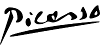
\includegraphics[scale=1]{signature.png}}{}% cache un blanc
\end{flushright} 
}

%%%%%%%%%%%%%%%%%%%%%%%%%%%%%
%% Note de frais seulement %%
%%%%%%%%%%%%%%%%%%%%%%%%%%%%%%%%%%%%%%%%%%%%%%%%%%%%%%%%%%%%%%%%%%%%%%%%%%%%%%%%%%%%%%%
%% Construit le titre Note de service de <mois> <annee>
\newcommand{\rsConstruitTitreEtDateNote}{
\begin{center} 
\textcolor{grisfonce}{{\Huge Note de frais}\\ {\rsmoisAnneeNote{}}}
\end{center}
}

